% Report on the 3x+1 Problem for Research Methods in Applied Maths
% 03.03.2020, Moritz Konarski, AUCA

%==============================================================================
% SETUP

\documentclass[12pt,a4paper,reqno]{amsart}

% packages used
\usepackage[english]{babel}
\usepackage[utf8]{inputenc}
\usepackage[T1]{fontenc}
\usepackage{amsmath}
\usepackage{amsfonts}
\usepackage{anysize}
\usepackage{textcomp}
\usepackage{graphicx}
\graphicspath{{../graphics/}}
\usepackage{epstopdf}
\usepackage[utf8]{inputenc}
\usepackage{fancyhdr}
\usepackage{lastpage}
\usepackage[hidelinks]{hyperref}
\hypersetup{
    colorlinks=true,
    linktoc=all,
    allcolors=black,
    final
}

% this command was found at:
% https://tex.stackexchange.com/questions/51851/change-distance-between-page-number-and-bottom-edge-of-page

\usepackage{calc}
\setlength{\footskip}{\paperheight
  -(1.25in+\voffset+\topmargin+\headheight+\headsep+\textheight)
  -1in}
\setlength{\headsep}{\voffset+\topmargin+\headheight + 0.3in}

% set line spacing
\renewcommand{\baselinestretch}{1.4}
% set margin size
\marginsize{1.25in}{1.25in}{1in}{1.5in}

%==============================================================================
% REPORT

%------------------------------------------------------------------------------
% TITLE PAGE AND ABSTRACT
% template can be found at:
% https://www.overleaf.com/learn/latex/How_to_Write_a_Thesis_in_LaTeX_(Part_5):_Customising_Your_Title_Page_and_Abstract

\begin{document}

\begin{titlepage}
    \begin{center}
        \vspace*{1cm}
            
        \Huge
        \textbf{An Overview of the $3x+1$ Problem}
            
        \vspace{0.5cm}
            
        \vspace{1.5cm}
            
        \LARGE
        \textbf{Moritz M. Konarski}
            
        \vfill
            
            
        \vspace{0.8cm}
            
        %\includegraphics[width=0.4\textwidth]{university}
            
        \Large
        Applied Mathematics Department\\
        American University of Central Asia\\
        Kyrgyzstan\\
        03.03.2020
            
    \end{center}
\end{titlepage}

\thispagestyle{plain}
\begin{center}
    \Large
    \textbf{An Overview of the $3x+1$ Problem}
        
    \vspace{0.4cm}
    \large
        
    \vspace{0.4cm}
    \textbf{Moritz M. Konarski}
       
    \vspace{0.9cm}
\end{center}
    \textsc{Abstract.} This paper gives an overview of the Collatz function, a 
    function that takes
    a positive integer as input and divides it by 2 if is even or multiplies
    it by 3 and adds 1. The Collatz conjecture states that this function, when
    repeatedly applied to itself, will eventually yield 1. This conjecture has
    been computationally verified to be correct for very large numbers, but the
    proof is still outstanding. The background and reasons to study the
    conjecture will be discussed. Furthermore, details of the $3x+1$ problem
    will be illustrated. Those details are trajectories, cycles, stopping time,
    and stochastic approximations. 

\tableofcontents

% this command was found at:
% https://tug.org/pipermail/texhax/2009-August/013136.html

\thispagestyle{empty}
\pagestyle{fancy}
\renewcommand{\headrulewidth}{0pt}

\fancyhead{}
\fancyhead[CE]{\textsc{Moritz M. Konarski}}
\fancyhead[CO]{\textsc{An Overview of the $3x+1$ Problem}}

%------------------------------------------------------------------------------
% INTRODUCTION

\section{Introduction}

The $3x+1$ Problem is a number theoretical problem that has been studied by 
mathematicians since the 1950s, but still
today it remains unsolved \cite{src:03}. This problem is defined in terms of
the \textit{Collatz function}, which, for any positive integer $x$, returns
$x/2$ if $x$ is even and $3x+1$ if $x$ is odd. Mathematicians study the
behavior of this function when it is repeatedly iterated, meaning it is applied
to itself. Following Lagarias \cite{src:03}, the Collatz function is defined as 

\begin{equation}
C(x)= \left\{
    \begin{array}{ll}
        3x+1 \quad &\text{if } x \equiv 1 \text{ (mod 2),} \\
        x/2 \quad &\text{if } x \equiv 0 \text{ (mod 2).}
    \end{array}
\right.
\label{eq:01}
\end{equation}

When the $3x+1$ Problem is studied, the \textit{$3x+1$ function} 

\begin{equation}
T(x)= \left\{
    \begin{array}{ll}
        (3x+1)/2 \quad &\text{if } x \equiv 1 \text{ (mod 2),} \\
        x/2 \quad &\text{if } x \equiv 0 \text{ (mod 2)}.
    \end{array}
\right.
\label{eq:02}
\end{equation}

The $3x+1$ function $T(x)$ 
takes integers as input and yields integers as outputs, making it a number
theoretic function like $C(x)$. More specifically, its
domain are all positive integers and its range are also the positive integers.
As such, $T(x)$ can be seen as the mapping of 
$\mathbb{N} + 1 \rightarrow \mathbb{N} + 1$, where $\mathbb{N} + 1$ represents
the positive integers \cite{src:04}. The $3x+1$ 
function is, like the Collatz function, repeatedly applied to itself and has 
a \textit{stopping time}, \textit{total stopping time}, and a 
\textit{trajectory} for each $x \in \mathbb{N} + 1$. \\
The $3x+1$ function is used instead of the Collatz function because it is more 
predictable \cite{src:03}. 
If $x$ is odd, $3x+1$ yields an even number that number is then 
immediately divided by 2. This has the effect that an otherwise following
iteration of $C(x)$ is not needed. Furthermore, the function cannot grow as
quickly because the factor is now $3/2$ instead of 3. These two changes make
the function easier to study \cite{src:03}.
Accordingly, $T(x)$ can alternatively be defined in terms of equation 
(\ref{eq:01}) as $C(x)$ if $x$ is even and as $C(C(x))$ if $x$ is odd:

\begin{equation}
T(x)= \left\{
\nonumber
    \begin{array}{ll}
        C(C(x))\quad &\text{if } x \equiv 1 \text{ (mod 2),} \\
        C(x) \quad &\text{if } x \equiv 0 \text{ (mod 2).}
    \end{array}
\right.
\label{eq:03}
\end{equation}

\subsection{The Collatz Conjecture}

\textit{For all $x \in \mathbb{N} + 1$ there is a $k \in \mathbb{N} + 1$ such 
that $T^{(k)}(x)=1$. For any positive integer $x$, $k$ iterations of the $3x+1$ 
function will yield the result 1.} \\
This conjecture has not yet been proven and remains of interest to
mathematicians who continue to study it to this day \cite{src:03}. According to 
Chamberland \cite{src:02}, because $T(x)$ is a number theoretical function, 
successive applications of $T(x)$ can have the following results:

\begin{enumerate}
    \item reach 1, which is equivalent to entering the trivial cycle,
        $\{2,1,2,1,\dots\}$
    \item enter a non-trivial cycle that does not include 1, or
    \item diverge to infinity and not enter any type of cycle.
\end{enumerate}

The Collatz conjecture states that point (1) is the only possible result and 
happens regardless of the positive integer that the iteration starts with.

\subsection{Background Information}

The Collatz conjecture and function are named after the German mathematician
Lothar Collatz. Collatz worked on problems similar to the $3x+1$ problem in the
early 1930s, according to Lagarias \cite{src:03}. The problem is also known as 
Hasse's Algorithm, Kakutani's Problem, and Ulam's Problem 
after other scientists who studied it or similar problems. During the 1950s 
the problem was circulated in various mathematical circles and the first 
publication was written about it in 1971 \cite{src:03}. \\
Today, the conjecture has been verified for over $10^{20}$ numbers using the 
help of computers to check if iterations of the $3x+1$ function eventually
reach 1 \cite{src:04}. A number that does not iterate to 1 has not yet been
found. \\
One of the most recent papers on the $3x+1$ problem, "\textit{Almost All Orbits
of the Collatz Map Attain Almost Bounded Values}" by Terence Tao \cite{src:04},
was published in September of 2019. He proved that almost all iterations of the
Collatz function are bounded, bringing mathematics one step closer to proving 
the Collatz conjecture. Currently, the problem is being actively researched.

\subsection{Reasons the Study the $3x+1$ Problem}

According to Lagarias \cite{src:03}, the fact that the problem is easy to state 
but hard to prove makes it an interesting challenge for mathematicians.
The fact that the $3x+1$ problem has remained unsolved after over 50 years
despite much research being done about it underlines the challenge. \\
One of the challenging aspects of this problem is the pseudo-random nature of 
the $T(x)$ function. The function is difficult to predict when it comes to how 
iterations of it will behave. Because mathematical proofs tend to rely on 
patterns, this pseudo-randomness makes a proof of the conjecture very
challenging. \\
Another reason for studying the $3x+1$ problem is that it can be studied as an 
iterative mapping of positive integers to positive integers. These kinds of
mappings are currently a popular research topic, according to Lagarias
\cite{src:03}. \\
Computer scientists also have an interest in the Collatz conjecture because 
the computational testing of its correctness is an important part of 
current research. Since the 1960s, computers have been used to verify if
positive integers follow the Collatz conjecture.
Because these calculations have verified the conjecture for over $10^{20}$ 
numbers \cite{src:04}, finding and optimizing computer algorithms is important. 
Furthermore, whether or not a given positive integer will iterate to 1 can be 
studied as a decision problem in computer science \cite{src:03}. \\
The study of prime numbers is also connected to the $3x+1$ problem and the
Collatz conjecture. If it were to be proven to be current, the proof may
further the understanding of prime factorization of integers. This is because 
the Collatz function, in a way, factors integers when dividing by 2. When odd 
numbers are multiplied by 3, another prime factor is introduced to the number.
The addition of 1 then can drastically change the way an integer can be
factored and accordingly this behavior is interesting to study \cite{src:03}.\\
Finally, when talking about this problem, mathematician Paul Erdös said that

\begin{quote}
Mathematics is not ready for such problems.
\end{quote}

If he is right and mathematics is indeed not ready for problems such as the
$3x+1$ problem, that could mean that new areas of mathematics are required to
prove or disprove it. A proof of the Collatz conjecture may thus involve new 
areas of mathematics or maybe require old areas to be applied in new and
different ways. Whatever the case may be, the $3x+1$ problem is an interesting
and challenging problem in mathematics and has connections to multiple other
areas of mathematics and computer science. If it were to be proven or
disproven, the effects could have wide-ranging implications \cite{src:03}.

\section{The $3x+1$ Problem in Detail}

This section will explain five main attributes connected to the $3x+1$ problem
and the study of the Collatz conjecture. First, trajectories of $T(x)$ will be
considered. Second, cycles of $T(x)$ will be considered. Then, the stopping
time and total stopping time of the $3x+1$ function are considered. Finally,
stochastic approximations of this function are explained.

\subsection{Trajectories}

The trajectory of $x$ under $T(x)$ is the set of the successive iterations of 
$T(x)$ that starts with $x$ and ends when $T^{(k)}(x)=1$. This means that the
trivial cycle $\{2,1,2,\dots\}$ is not included. This makes sense because
otherwise all trajectories would be infinite in length. Accordingly, the 
trajectory of $T(x)$ has the length $k+1$ because the first element of the 
trajectory $x$ has the iteration number $k=0$. Trajectories are also called 
forward orbits $O^+(x)$ of $x$ under $T(x)$. Following Chamberland
\cite{src:02}, the trajectory of $x$ under $T(x)$ is defined as 

\begin{equation}
    \nonumber
    O^+(x):=\{x, T(x), T^{(2)}(x), T^{(3)}(x),\dots\}
\end{equation}

These trajectories contain all the numbers that the iteration of $T(x)$ yields. 
They can be graphed to illustrate what $T(x)$ does when repeatedly iterated. 
Looking at graphs of trajectories illustrates why $T(x)$ is considered
a pseudo-random function, its erratic behavior is evident \cite{src:03}.

\subsection{Cycles}

Cycles of $T(x)$ are sequences of iterations of $T(x)$ that periodically 
repeat. It is known that $T(x)$ has the trivial cycle $\{2,1,2,\dots\}$, which 
is equivalent to reaching 1. Because of this equivalence, the trivial cycle is
not included in the trajectories because it never ends and the resulting values
don't leave the cycle. The Collatz conjecture states that any initial positive 
integer $x$ will, after $k$ iterations of $T(x)$, enter this trivial cycle. 
This means that the trivial cycle is the only cycle that can exist if the
Collatz conjecture is true.
In case non-trivial cycles do exist, which would disprove the Collatz
conjecture, it has been proven that those non-trivial cycles must be more than 
10.4 billion numbers long. \\
The $3x+1$ function can also be applied to all integers. When this is done, it
results in three more cycles, which, together with the trivial cycle, are 
conjectured to be the only ones that exist for $x \in \mathbb{Z}$. These 
cycles start at -1, -5, and -17.

% TODO: decide whether or not to keep this equation in
\begin{align} \nonumber
    O^+(-1)=\{ &-1, -1, -1, -1\}, \\ \nonumber
    O^+(-5)=\{ &-5, -7, -10, -5\}, \\ \nonumber
    O^+(-17)=\{&-17, -25, -37, -55, -82, -41, \\ \nonumber
               &-61, -91, -136, -68, -34, -17\}
\end{align}

\subsection{Stopping Time}

The stopping time of $T(x)$ is the number of iterations $k$ of $T(x)$ that it takes
for the result of an iteration to be less than $x$. This is called stopping 
time because as soon as $x > T^{(k)}(x)$ it is known that the iteration will
reach 1 and \textit{stop}. Additionally, reaching this stopping point means
that we can stop to check if an iteration reaches one. To be able to apply this 
stopping time, all numbers 
up to and including $x-1$ have to be verified to iterate to 1. Then, if $T^{(k)}(x) < x$, 
it is obvious that $T(x)$ will also iterate to 1. The reason for that is that
the trajectory of $T(x)$ is always the same and it contains some trajectories
of other numbers. If we know that one of the numbers in the trajectory of
$T(x)$ iterates to one, we know that $T(x)$ does so too.
The stopping time of $x$ is called $\sigma(x)$ and defined as

\begin{equation}
    \nonumber
    \sigma(x)=\inf\{k:T^{(k)}(x) < x\}.
\end{equation}

Defining it like this
makes sense because if one checks integers for compliance, it makes sense to
start small and work towards larger integers. Furthermore, because, on average,
the value of $T(x)$ decreases, this definition makes a lot of sense. This 
abbreviation makes it simple to check if a particular number iterates to 1 and
saves a lot of computations that have already been performed. If the Collatz 
conjecture is true, all $x \in \mathbb{N} + 1$ have a finite stopping time, 
meaning they iterate to 1 eventually. \\
Related to the stopping time $\sigma(x)$ is the total stopping time
$\sigma_{\infty}(x)$. This is the total number of iterations needed for $T(x)$ 
to iterate to 1. It is defined as

\begin{equation}
    \nonumber
    \sigma_{\infty}(x)=\inf\{k:T^{(k)}(x)=1\}.
\end{equation}

The total stopping time of $T(x)$ is conjectured to be finite for all $x \in
\mathbb{N} + 1$ as a direct result of the Collatz conjecture.

\subsection{Stochastic Approximations}

When looking at the values that individual iterations of $T(x)$ yield,
mathematicians noticed that for the trajectories of large numbers, the number
of odd and even numbers is approximately the same.
% TODO: show a graph to illustrate this
Furthermore, they observed
that $T(x)$ behaves pseudo-randomly, meaning that it is hard to predict which
value the function will take on in one or two iterations. Mathematicians use
this property of $T(x)$ to make probabilistic statements about groups of
trajectories and study their behaviors in this way. For example, the upper
bound of for the total stopping time has been proven to be $41.677647 \log x$
\cite{src:03}. \\
One useful application of these stochastic approximations is the approximation
of the total stopping time of $T(x)$. The total stopping time for most 
trajectories is approximated to be $6.95212 \log x$ steps. 

\section{Examples}

\subsection{$3x+1$ Function for $x=39$}

\begin{itemize}
    \item trajectory
    \item graph
    \item stopping time
    \item total stopping time
    \item total stopping time approximation
    \item even and odd numbers counted
\end{itemize}

With the trajectory of $T(39)$ being

\begin{align}
    \nonumber
    O^+(39):=\{&39,59,89,134,67,101,152,76,\textbf{38},19,29,\\
    \nonumber
               &44,22,11,17,26,13,20,10,5,8,4,2,1\},
\end{align}

we see that 38 is the first number <39. If we have previously shown that
$T(38)$ iterates to 1, we can infer that $T(39)$ does so too. Thus 
$\sigma(39) = 8$, as 38 is the result of the 8th iteration.
% TODO: give stopping time for 27
\subsubsection{The trajectory of $T(39)$}

The trajectory of $T(39)$ is
\begin{align}
    \nonumber
    O^+(39):=\{&39,59,89,134,67,101,152,76,38,19,29,\\
    \nonumber
               &44,22,11,17,26,13,20,10,5,8,4,2,1\}
\end{align}
When graphed, one can see that $T^{(k)}(39)$ increases and decreases in
a seemingly random manner.
\begin{figure}[h]
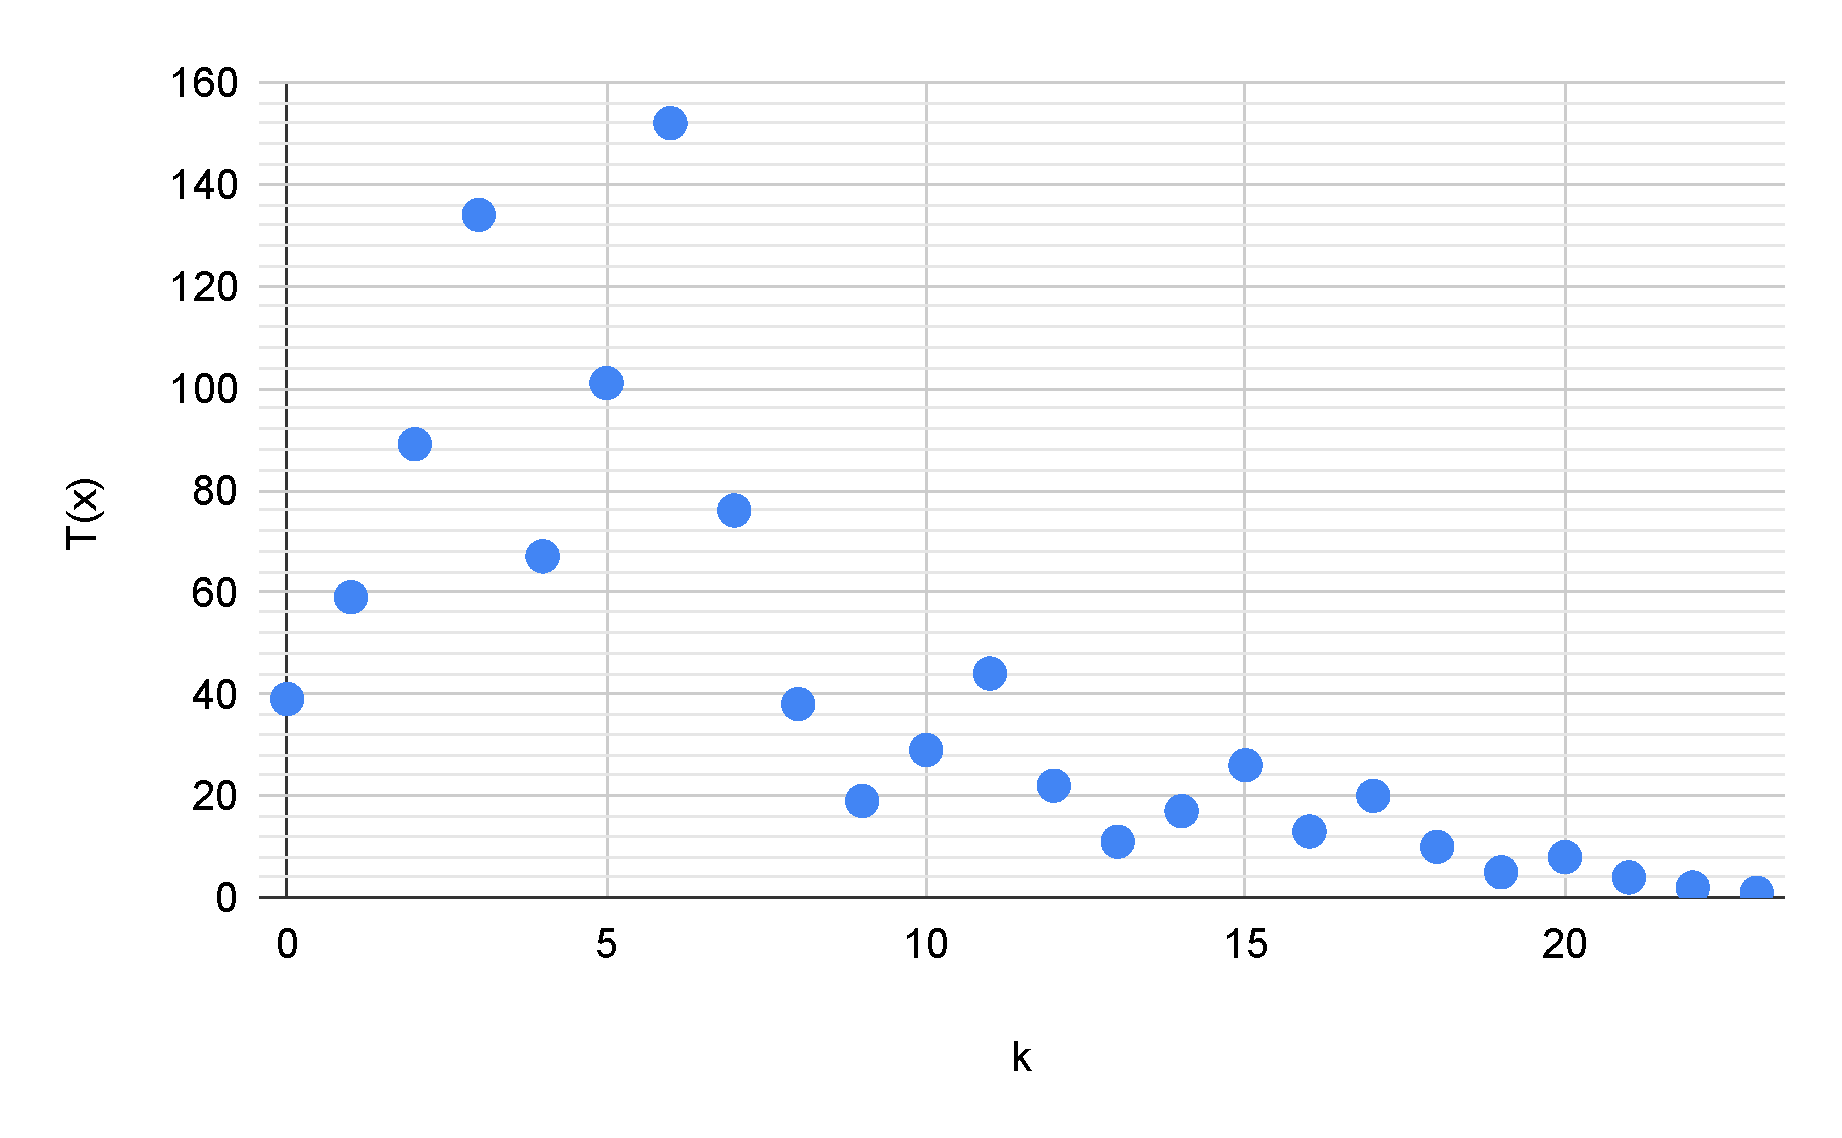
\includegraphics[width=\textwidth]{39-8-23}
    \caption{The trajectory of $T^{(k)}(39)$ by number of iterations}
\label{fig:01}
\end{figure}

For $T(39)$ we have the approximation
\begin{equation}\nonumber
    6.95212 \log 39 \approx 25.4952
\end{equation}
Compared to the known $\sigma_{\infty}(39)=23$ this is not bad.

For $T(39)$, which we considered above, 
\begin{align}
    \nonumber
    O^+(39):=\{&39,59,89,134,67,101,152,76,38,19,29,\\
    \nonumber
               &44,22,11,17,26,13,20,10,5,8,4,2,1\}
\end{align}
and we see that $T^{(23)}(39)=1$, this means that it takes 23 iterations of
$T(x)$ to iterate to one. Accordingly, $\sigma_{\infty}(39)=23$.

\subsection{$3x+1$ Function for $x=27$}

\begin{itemize}
    \item trajectory
    \item graph
    \item stopping time
    \item total stopping time
    \item total stopping time approximation
    \item even and odd numbers counted
\end{itemize}

\begin{figure}[h]
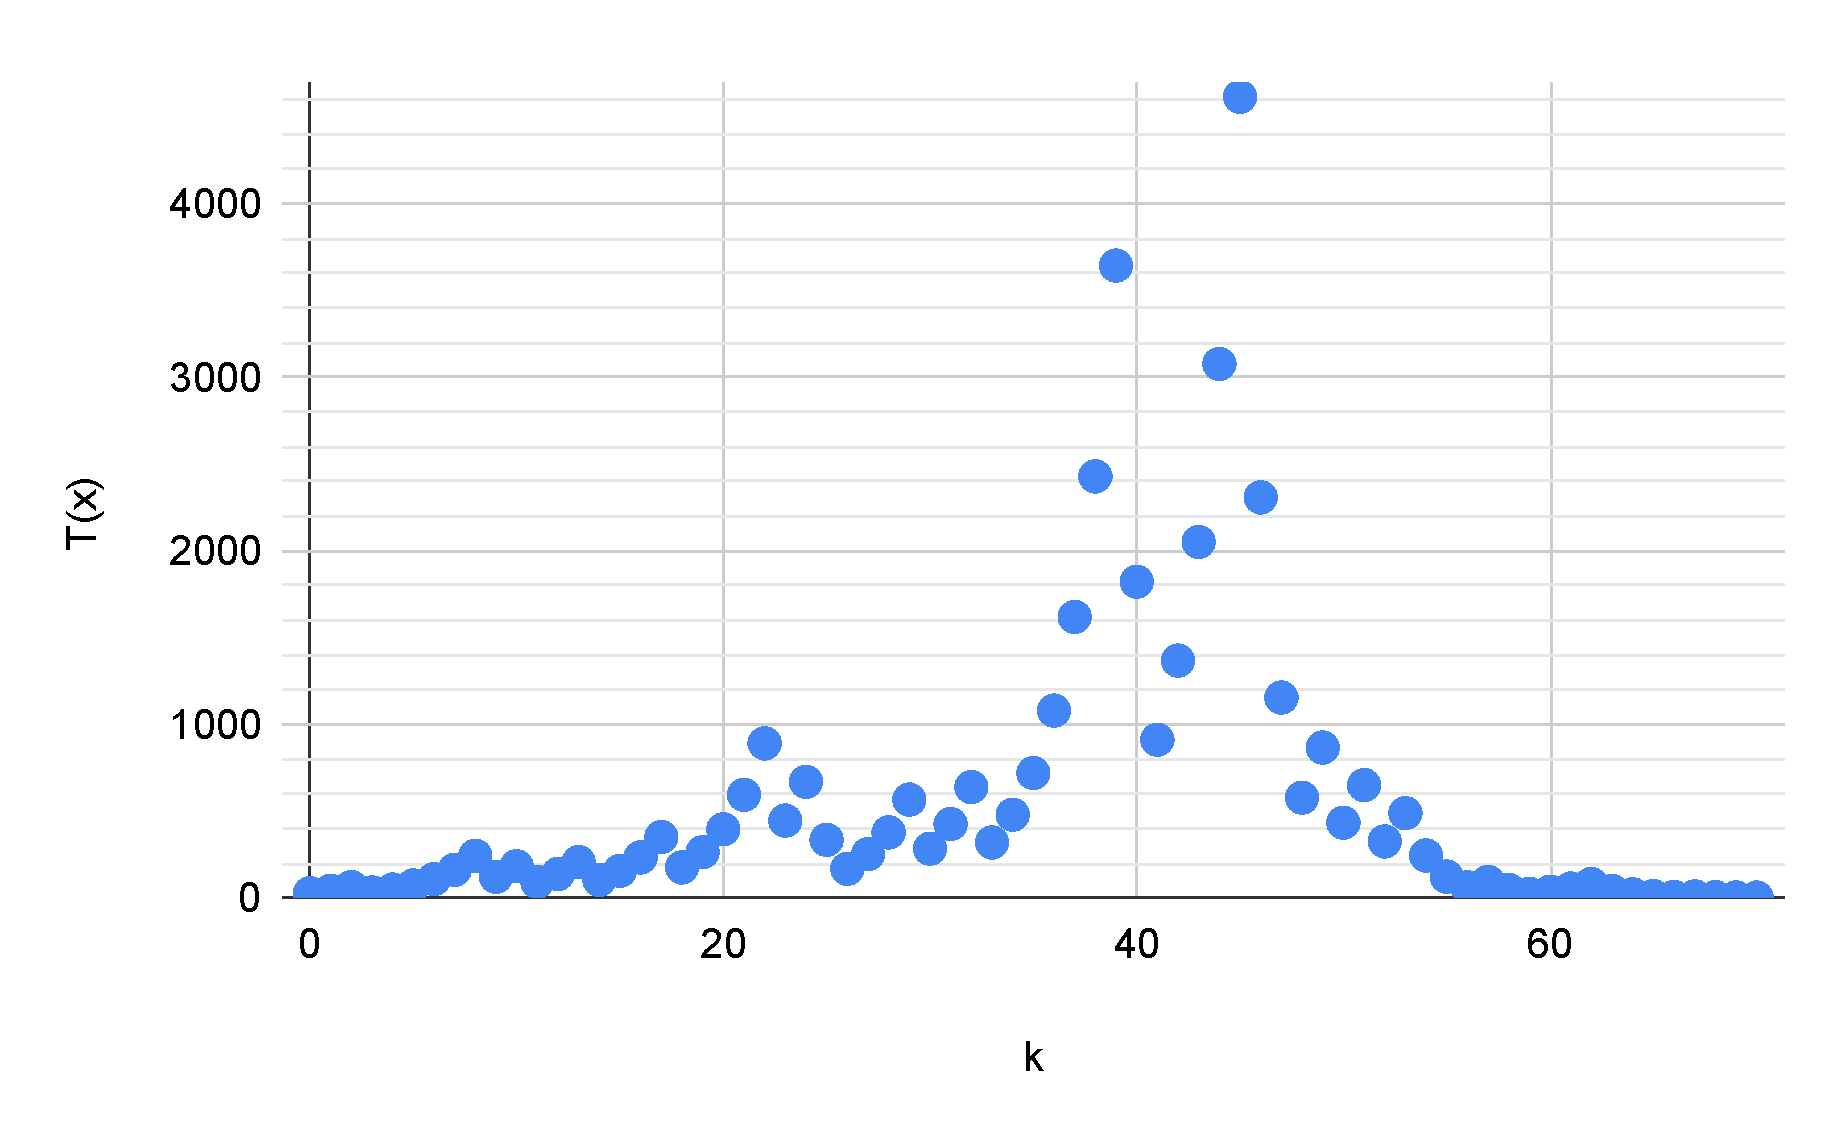
\includegraphics[width=\textwidth]{27-59-70}
    \caption{The trajectory of $T^{(k)}(27)$ by number of iterations}
\label{fig:02}
\end{figure}

\subsection{$3x+1$ Function for $x=489$}

\begin{itemize}
    \item trajectory
    \item graph
    \item stopping time
    \item total stopping time
    \item total stopping time approximation
    \item even and odd numbers counted
\end{itemize}

\begin{figure}[h]
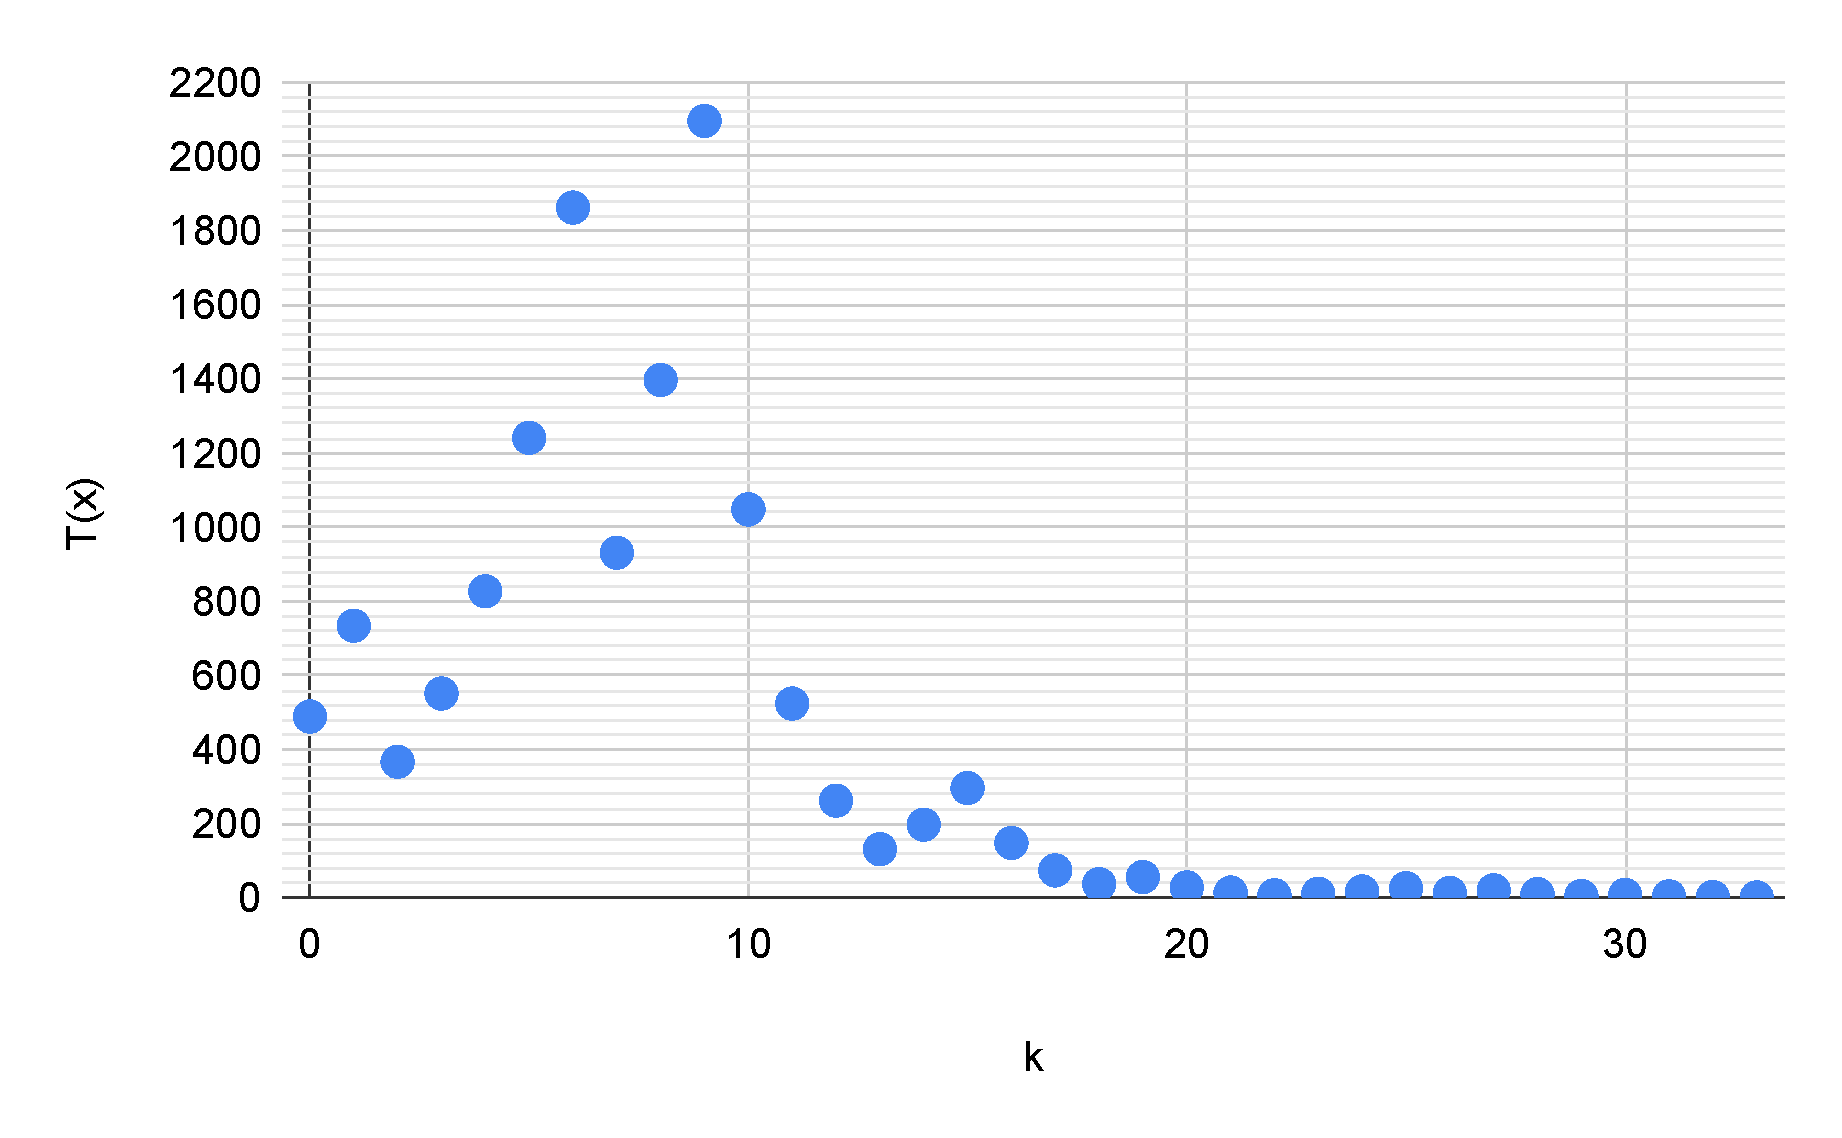
\includegraphics[width=\textwidth]{489-2-33}
    \caption{The trajectory of $T^{(k)}(489)$ by number of iterations}
\label{fig:03}
\end{figure}


\section{Conclusion}

\begin{itemize}
    \item the Collatz Conjecture states that for $x,k \in \mathbb{N} + 1$
        $T^{(k)}(x)=1$
    \item the conjecture has not been proven, but verified for $10^{20}$
        numbers
    \item pseudo-random nature
    \item relation to other fields of maths
    \item all orbits of $T(x)$ should reach the trivial cycle
    \item $T(x)$ can be probabilistically described because of pseudo-randomness
\end{itemize}


%==============================================================================
% BIBLIOGRAPHY

\begin{thebibliography}{4}

\bibitem{src:01} Marc Chamberland, 
    \textit{An Update on the $3x+1$ Problem},
    \texttt{http://www.math.grinnell.edu/\\
        \~{}chamberl/papers/3x\_survey\_eng.pdf}, 2005.

\bibitem{src:02} R. E. Crandall, \textit{On the "$3x+1$" Problem},
    Mathematics of Computation, \textbf{32} (1978), no. 144, 1281-1292.

\bibitem{src:03} Jeffrey C.Lagarias, 
    \textit{The $3x+1$ Problem: An Overview},
    \texttt{https://pdfs.semanticscholar.\\
        org/100046dd8b4ee901bc71043da7d42f5d87ca0224.pdf}, 2010.

\bibitem{src:04} Terence Tao, \textit{Almost All Orbits of the Collatz Map Attain
    Almost Bounded Values}, arXiv:1909.03562v2 [math.PR], 2019.

\end{thebibliography}
\end{document}
